The rock block generating algorithm is based on a subdivision approach: each discontinuity is introduced sequentially and if it intersects the parent block, the parent block is subdivided into two child blocks. This process is repeated until all discontinuities have been processed and is repeated for each block. Figure \ref{fig:SlicingIllustration} shows a simple schematic of this process. The original serial algorithm is implemented in C++ using data structures to represent the blocks and discontinuities. \par

\begin{figure}[h]
  \centering
  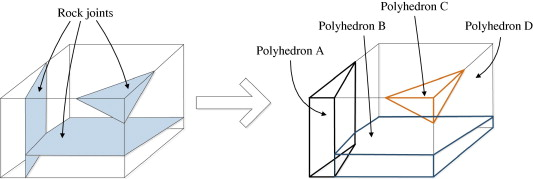
\includegraphics[width=0.4\textwidth]{SlicingIllustration}
  \caption{Polyhedron generation schematic \cite{slicing}}
  \label{fig:SlicingIllustration}
\end{figure}

This algorithm is refactored and modified in Scala to run in parallel on Spark using a functional approach. The following sections give a description of how the different stages of the rock generation process are implemented from a high level. Section 3 gives more detail on the actual code generated to do this.  Within Scala, the blocks are case classes that keep a list of faces that define the block as well as the location of its center in global coordinates. The faces are are objects that store the face's normal vector, a distance from the block's origin, as well as the friction angle and cohesion along the face. The discontinuities, or joints, are also case classes. The class contains the normal vector to the plane that defines the joint, its distance from the joint's local origin and the global coordinates that define that origin. Additionally, it stores the dip angle, dip direction (shown in Figure \ref{fig:DipFig}), friction angle and cohesion along the joint face. In the case of non-persistent joints, it also stores a list of inequalities that describe the shape of the joint.

\begin {figure}[h]
  \centering
  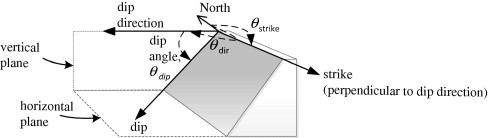
\includegraphics[width=0.4\textwidth]{DipFig}
  \caption{Definition of strike, dip and dip direction \cite{slicing}}
  \label{fig:DipFig}
\end{figure}

Using this data structure, it is possible to completely describe the volume defining a polyhedral block, negating the need to story any information on the edges and vertices which can be calculated if necessary. The volume defining a block bounded by \textit{N} planes can be described completely by the following inequality:
\begin{equation}
a_ix + b_iy + c_iz \leq d_i, \; i = 1 ,\, \ldots ,\, N
\end{equation}

The coefficients $(a_i, b_i, c_i)$ represent the normal vector to the $i^{th}$ plane bounding the block and $d_i$ is the distance of that plane from some local origin. \par
 
In order to subdivide a block, it is necessary to establish whether the block is intersected by the discontinuity being considered. The novelty in the algorithm presented in \cite{slicing} is recasting this problem as the following linear program: 
\begin{equation}
\begin{aligned} 
&\text{minimize } s\\
&\boldsymbol{a_{i}^{T} x} - d_i \leq s, i = 1,...,N\\
&\boldsymbol{a_{\text{new}}^{T} x} - d_{\text{new}} = 0
\end{aligned}
\end{equation}

Here \textit{N} represents the number of planes that define the block and the discontinuity being considered is represented by the equality. If $s < 0$, there is an intersection and the parent block is split into two child blocks. The child blocks inherit all parent block's planes as well as the intersecting discontinuity with opposite signs for each child block. \par

As the subdivision continues, some of the discontinuities may become geometrically redundant. It is not necessary to remove these redundancies after each intersection check; instead they can be removed after all discontinuities have been considered. Again, this can be done by solving a linear program: 
\begin{equation}
\begin{aligned}
&\text{maximize }\boldsymbol{c^{T} x}\\
&\boldsymbol{a_{i}^{T} x} - d_{i}, i = 1,...,N
\end{aligned}
\end{equation}

Here, \textbf{c} is one of the normal vectors $a_{i}$. If $\vert \boldsymbol{c^{T} x} - d \vert < \varepsilon$ is true the discontinuity is redundant, where $\varepsilon$ represents numerical tolerance close to zero. \par

Not all joints are necessarily persistent, i.e. not all joints extend through the entire rock mass, and this needs to be accounted for in the solution of the linear program. Each joint contains a list of inequalities that represent its extent within the plane that defines the joint. These inequalities are in reference to a local origin within the joint plane and first need to be converted to global coordinates before intersection can be established. The local inequalities are transformed to global coordinates through a rotation transformation to then yield the following linear program: 
\begin{equation}
\begin{aligned} 
&\text{minimize } s\\
&\boldsymbol{a_{i}^{T} x} - d_i \leq s, i = 1,...,N\\
&\boldsymbol{a_{\text{new}}^{T} x} - d_{\text{new}} = 0\\
&\boldsymbol{a_{j,\text{bound}}^{T} x} - d_{j,\text{bound}} = 0
\end{aligned}
\end{equation}

The additional constraints sub-scripted with \textit{bound} define the boundaries of the \textit{new} discontinuity. 

After each discontinuity has been processed by each block and all redundant joints have been removed, the final result is a list of \textit{Block} objects. The final step before outputting the results is to find the centroid of each block. In order to do this, it is necessary to calculate the vertices but this is only done once throughout all the computations. Using the vertex coordinates, each face is meshed using Delaunay triangulation. By doing this, the entire boundary of the polyhedron is described as a union of triangles that can then be used to find the centroid as outlined in \cite{centroid}. 

\subsection{Input Processing}
The input data consists of all the faces that define the rock volume of interest as well as all the joints that intersect this volume. The distances of the faces and joints are all relative to a global origin. The input format is a multi-line text file where each line contains the relevant input for either a face or a joint. The input ordering should be such that all faces that define the rock volume occur first in the text file. While reading the input, if a line with a single ``\%'' is encountered, the input reading switches to joints. \par

Additionally, the joints should be ordered in sequence according to their mechanical genesis so that blocks generated represent patterns observed in the field. Persistent joints should be introduced first to ensure that enough blocks are generated to seed the initial resilient distributed data set (RDD) in Spark. Unless all joints are persistent, the order in which joints are introduced will have an impact on the shape and pattern of blocks generated. Careful consideration must be given the rock type being analyzed as its formation and geologic history will guide how the joints should be introduced in the algorithm. \par

\subsection{Processing Discontinuities}
Before creating an RDD, the same number of joints is processed as the number of cores in the submitted job. This allows for sufficient blocks to be generated to seed the initial RDD. As discussed later, how the RDD is seeded will have a significant impact on load balancing. \par

Once these joints have been processed, a Spark context is started and the initial RDD is created. The list of remaining joints is broadcast to all nodes in the cluster and the discontinuities can be processed in parallel. Each node iterates through the list of joints and checks whether it intersects the blocks in its RDD. This is done by using \texttt{flatMap} on the \texttt{cut} method for each block. This method solves the linear program described above to determine intersection - the open-source linear program solver \texttt{lp\_solve} \cite{lpsolve} is called within the method to do this. If the joint intersects a block, two child blocks are generated and added to the node's RDD. If there is no intersection, the RDD remains unchanged and the next joint processed.

\subsection{Redundant Joints}
After all joints in the data set have been processed, the redundant joints are removed from the list of faces for all blocks. This is achieved in parallel by mapping a \texttt{nonRedundantFaces} method defined in the \textit{Block} class across the RDD. This method returns a new \textit{Block} object that contains only the non-redundant faces. Using a functional approach and pattern matching, a new list containing all the blocks in the RDD is generated when removing the redundant joints.

\subsection{Calculate Centroids}
Before finalizing the list of blocks, it is necessary to calculate their centroids since this is required for a typical discrete element analysis. This requires knowledge of the blocks' vertices. The vertices are calculated by iterating over the list of faces, solving a $3x3$ system for all possible combinations. 

To calculate the centroid following \cite{centroid}, the boundary of the block must be described as a union of triangles. The most efficient way to divide the boundaries of the block is by dividing the faces into triangles and since we know the vertices it lends itself to Delaunay triangulation. Instead of doing the triangulation in three dimensions, the faces are rotated to a two-dimensional local coordinate system and then meshed. This ensures that the ordering of the nodes is consistently counter-clockwise which is necessary for the centroid calculations. We used an existing Dealaunay triangulation library implemented in Scala \cite{delaunay}.

All of the calculations mentioned above are implemented as methods within the \textit{Block} class. Again, the functional approach lends itself to \textit{map} and pattern matching on Spark: the vertices are calculated using \texttt{findVertices} which then are fed into the \texttt{mesh} method. The vertices and mesh then serve as the inputs to \textit{centroid}. The calculated centroid is used to find the new distances of the faces relative to the centroid in \texttt{updateFaces}. The centroid and updated faces are then the inputs to the \textit{Block} constructor, so a list of new blocks is returned with the correct centroids and faces when the mapping is completed.

\subsection{Output to JSON}
The final list of blocks is then ready to be used in a DEM analysis. In order to make the output accesible to other software, the resulting list of blocks is printed in JSON format to a text file. This is achieved through a \textit{json} object that contains methods for converting the \textit{Block}data structure to JSON and then writing the converted data to a text file. 
